\documentclass[11pt]{article}

\usepackage[a4paper,margin=1in]{geometry}
\usepackage{amsmath,amssymb}
\usepackage{graphicx}
\usepackage{booktabs}
\usepackage{hyperref}
\usepackage{microtype}

\hypersetup{
    pdftitle={Spherical Chamfer Generative Networks: One-Step Continuous Text-Conditional Generation by Joint Hypersphere Matching},
    pdfauthor={Ivan Shivalov},
    pdfsubject={Machine learning; conditional generative modeling},
    pdfkeywords={generative modeling, Chamfer distance, hypersphere, conditional generation, one-step generation},
    colorlinks=true,
    linkcolor=blue,
    citecolor=blue,
    urlcolor=blue
}

\title{Spherical Chamfer Generative Networks:\\
One-Step Continuous Text-Conditional Generation by Joint Hypersphere Matching}

\author{
Ivan Shivalov\\
Independent Researcher\\
\texttt{ivansivalov396@gmail.com}\\
\url{https://github.com/intexcor/SCGN}
}

\date{May 31, 2026}

\begin{document}
\maketitle

\begin{abstract}
We introduce Spherical Chamfer Generative Networks (SCGN), a simple one-step
conditional image generation prototype trained without adversarial losses,
diffusion sampling, paired reconstruction, or explicit optimal-transport
solvers. The method maps random noise and a continuous conditioning vector
directly to an image in a single forward pass. Its core constraint is geometric:
generated and real images are projected onto a fixed-radius hypersphere, and
training minimizes a bidirectional Chamfer objective in a joint space formed by
image direction and condition direction. The hyperspherical projection prevents
the trivial low-variance mean solution that appears under naive pixel matching,
while the joint image-condition nearest-neighbor loss encourages conditional
routing without class-classification losses. We report preliminary qualitative
results on MNIST, Fashion-MNIST, CIFAR-10, and a synthetic text-encoder mode in
which each image receives a unique prompt embedding. This technical report is
intended to document the method and its initial empirical behavior; large-scale
evaluation and comparisons are left for future work.
\end{abstract}

\section{Introduction}
Modern image generators are typically trained with one of several powerful but
complex mechanisms: adversarial discrimination \cite{goodfellow2014generative},
multi-step diffusion or score-based sampling \cite{ho2020denoising,
song2021score}, flow or transport-based objectives \cite{lipman2022flow,
liu2022flow}, or explicit optimal-transport approximations such as Sinkhorn
iterations \cite{cuturi2013sinkhorn}. These approaches have produced strong
results, but they also introduce either unstable adversarial dynamics,
computationally expensive iterative sampling, or nontrivial matching machinery.

This report explores a deliberately small alternative. SCGN trains a generator
$G_\theta(z,c)$ that maps a random vector $z$ and a continuous condition
embedding $c$ directly to an image. Instead of asking the generator to match
each training example with a fixed reconstruction target, SCGN treats each
minibatch as two unordered sets: generated samples and real samples. The sets
are matched through a bidirectional Chamfer objective, but the matching cost is
computed in a joint space that combines image similarity and condition
similarity.

The main idea is that naive pixel-space set matching is underconstrained:
averaging many possible targets can produce low-contrast ``gray'' outputs or
mode collapse. SCGN adds a hyperspherical image constraint. Both generated and
real images are compared only through their normalized directions, and generated
images are explicitly projected to the sphere of radius
$R=\sqrt{C H W}$. This removes the origin and low-norm averages as easy
solutions and forces the generator to maintain nontrivial contrast.

Our contribution is not a finished large-scale generative model. It is a compact
training principle:
\begin{enumerate}
    \item project images to a fixed-radius hypersphere;
    \item define a joint image-condition cosine cost;
    \item optimize a bidirectional Chamfer objective over minibatch sets;
    \item generate in one forward pass without adversarial, diffusion, paired
    reconstruction, or explicit transport-solver machinery.
\end{enumerate}

\section{Method}
\subsection{Generator and Conditioning}
Let $x \in \mathbb{R}^{C \times H \times W}$ be an image and
$c \in \mathbb{R}^{d_c}$ be a continuous condition vector. SCGN uses a neural
generator
\begin{equation}
    \hat{x}_i = G_\theta(z_i, c_i),
    \qquad z_i \sim \mathcal{N}(0,I),
\end{equation}
where $z_i$ is normalized before being concatenated with the condition vector.
The implementation used in this report is a small convolutional upsampling
network with residual blocks.

For conditional experiments we use two modes. In the first, each class label is
mapped to a fixed random normalized embedding. In the second, a minimal
bag-of-words text encoder is trained jointly with the generator. Each training
condition contains a class token and a randomly sampled adjective token, so the
condition vector is continuous and each prompt instance can be unique.

\subsection{Hyperspherical Image Projection}
For an image tensor $x$, define its flattened vector as
$v(x)\in\mathbb{R}^{D}$, where $D=CHW$. We compare image directions by
\begin{equation}
    \bar{x} = \frac{v(x)}{\|v(x)\|_2}.
\end{equation}
Generated images are also projected to a fixed radius:
\begin{equation}
    G_\theta(z,c) \leftarrow
    R \frac{v(G_\theta(z,c))}{\|v(G_\theta(z,c))\|_2},
    \qquad R=\sqrt{D}.
\end{equation}
This projection is intended to prevent collapse toward the origin or toward
low-variance pixel averages. It turns the image component of training into an
angular matching problem.

\subsection{Joint Spherical Chamfer Objective}
Given a minibatch of generated samples
$\{(\hat{x}_i,\hat{c}_i)\}_{i=1}^{B}$ and real samples
$\{(x_j,c_j)\}_{j=1}^{B}$, define image and condition cosine similarities:
\begin{align}
    s^{img}_{ij} &= \bar{\hat{x}}_i^\top \bar{x}_j,\\
    s^{cond}_{ij} &= \bar{\hat{c}}_i^\top \bar{c}_j.
\end{align}
The joint matching cost is
\begin{equation}
    C_{ij} =
    (1 - s^{img}_{ij}) + \gamma(1 - s^{cond}_{ij}),
\end{equation}
where $\gamma$ controls the strength of conditional alignment.

SCGN minimizes the bidirectional Chamfer loss
\begin{equation}
    \mathcal{L}_{SCGN}
    =
    \frac{1}{B}\sum_{i=1}^{B}\min_j C_{ij}
    +
    \frac{1}{B}\sum_{j=1}^{B}\min_i C_{ij}.
\end{equation}
The first term asks every generated sample to find a compatible real neighbor.
The second term asks every real sample to be covered by at least one generated
sample. Unlike a paired reconstruction loss, the nearest-neighbor assignment is
computed dynamically inside each minibatch. Unlike Sinkhorn or Hungarian
matching, the objective uses only row-wise and column-wise minima.

\section{Implementation}
The reference implementation is intentionally short. The essential training
step is:
\begin{verbatim}
sim_img = torch.mm(gen_img_norm, real_img_norm.t())
sim_cond = torch.mm(gen_cond, real_cond.t())
C = (1.0 - sim_img) + gamma * (1.0 - sim_cond)
loss = C.min(dim=1)[0].mean() + C.min(dim=0)[0].mean()
\end{verbatim}
All experiments in this preliminary report use $32\times32$ images, Adam with
learning rate $2\cdot10^{-4}$, batch size 128, latent dimension 128, condition
dimension 64, and $\gamma=5$ unless otherwise noted. The code is available at
\url{https://github.com/intexcor/SCGN}.

\section{Preliminary Experiments}
\subsection{Datasets}
We test the prototype on MNIST, Fashion-MNIST, and CIFAR-10. MNIST and
Fashion-MNIST are resized to $32\times32$ and treated as one-channel images.
CIFAR-10 is trained as a three-channel image dataset. The results reported here
are qualitative samples from the current prototype, not a full benchmark.

\begin{table}[h]
\centering
\caption{Preliminary experimental settings.}
\begin{tabular}{llll}
\toprule
Dataset & Resolution & Channels & Conditioning mode \\
\midrule
MNIST & $32\times32$ & 1 & fixed continuous label embedding \\
MNIST & $32\times32$ & 1 & jointly trained synthetic text encoder \\
Fashion-MNIST & $32\times32$ & 1 & fixed continuous label embedding \\
CIFAR-10 & $32\times32$ & 3 & fixed continuous label embedding \\
\bottomrule
\end{tabular}
\end{table}

\subsection{Qualitative Samples}
Figure~\ref{fig:samples} shows samples produced by the current implementation.
The MNIST runs show recognizable digit structure under both fixed continuous
label embeddings and the synthetic text-encoder mode. Fashion-MNIST shows
coherent clothing-like silhouettes. CIFAR-10 remains less mature but indicates
that the same objective can be applied to natural-image RGB data.

\begin{figure}[t]
\centering
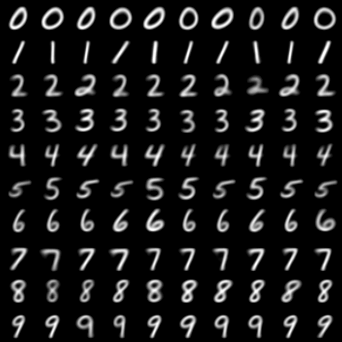
\includegraphics[width=0.48\linewidth]{figures/mnist_dummy.png}
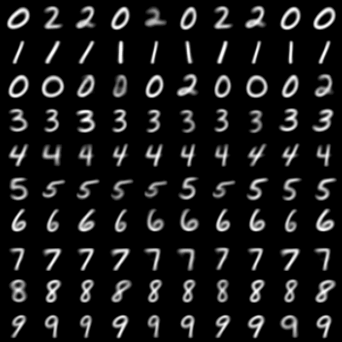
\includegraphics[width=0.48\linewidth]{figures/mnist_text_encoder.png}\\
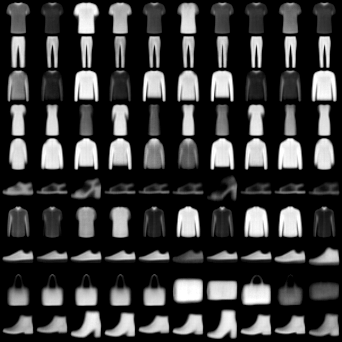
\includegraphics[width=0.48\linewidth]{figures/fmnist.png}
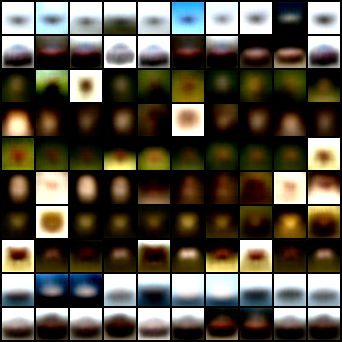
\includegraphics[width=0.48\linewidth]{figures/cifar10.png}
\caption{Preliminary SCGN samples. Top left: MNIST with fixed continuous
label embeddings. Top right: MNIST with jointly trained synthetic text-encoder
conditions. Bottom left: Fashion-MNIST. Bottom right: CIFAR-10.}
\label{fig:samples}
\end{figure}

\section{Discussion}
\paragraph{Why the sphere matters.}
The hyperspherical projection changes the failure modes of direct pixel-space
matching. A low-contrast average image has small angular distinctiveness and is
not an attractive way to cover many real samples on the sphere. The generator is
therefore biased toward high-variance outputs that lie on the same norm shell
as normalized real images.

\paragraph{Why joint matching matters.}
Pure image-space Chamfer matching does not identify which condition should map
to which visual structure. Adding condition cosine distance to the matching cost
makes generated samples compete for real samples with compatible condition
vectors. In practice this acts as a routing signal without requiring an
auxiliary classifier loss.

\paragraph{Relation to optimal transport.}
The objective resembles set matching, but it does not solve a balanced
transport problem. There is no transport plan, entropy regularization, Sinkhorn
iteration, or Hungarian assignment. The method uses nearest-neighbor coverage in
both directions as a lightweight surrogate.

\section{Limitations and Future Work}
This report is intentionally preliminary. The current evidence is qualitative
and does not yet include FID, KID, precision-recall, classifier-based
conditional alignment, or nearest-neighbor memorization tests. The text-encoder
experiment uses synthetic prompts rather than a pretrained language-image model,
so it should be read as evidence for continuous conditioning and routing rather
than as proof of open-vocabulary text-to-image generation.

Important next steps include:
\begin{enumerate}
    \item ablations without hyperspherical projection, without the condition
    term, and with one-way instead of bidirectional Chamfer;
    \item sweeps over $\gamma$, batch size, latent dimension, and condition
    dimensionality;
    \item quantitative evaluation on held-out test data;
    \item nearest-neighbor analysis to measure memorization;
    \item replacement of the synthetic text encoder with pretrained CLIP or T5
    embeddings.
\end{enumerate}

\section{Conclusion}
SCGN is a compact geometric prototype for one-step conditional generation. By
combining hyperspherical image projection with a joint image-condition Chamfer
objective, the method trains a generator without adversarial losses, diffusion
sampling, paired reconstruction, or explicit transport solvers. The preliminary
results suggest that this direction is worth deeper study, especially as a
minimal set-matching objective for fast conditional generation.

\section*{Acknowledgements}
No external funding was used.

\bibliographystyle{plain}
\bibliography{references}

\end{document}
